\documentclass[xetex,mathserif,serif]{beamer}
\usepackage{polyglossia}
\setdefaultlanguage[babelshorthands=true]{russian}
\usepackage{minted}
\usepackage{tabu}
\usepackage{moresize}

\useoutertheme{infolines}

\usepackage{fontspec}
\setmainfont{FreeSans}
\newfontfamily{\russianfonttt}{FreeSans}

\definecolor{links}{HTML}{2A1B81}
\hypersetup{colorlinks,linkcolor=,urlcolor=links}

\tabulinesep=1.2mm

\title{Практика по Java}
\subtitle{Введение}
\author[Юрий Литвинов]{Юрий Литвинов\\\small{\textcolor{gray}{yurii.litvinov@gmail.com}}}
\date{16.01.2019г}

\newcommand{\attribution}[1] {
\vspace{-5mm}\begin{flushright}\begin{scriptsize}\textcolor{gray}{\textcopyright\, #1}\end{scriptsize}\end{flushright}
}

\begin{document}

	\frame{\titlepage}

	\section{Введение}

	\begin{frame}
		\frametitle{Формальности}
		\begin{itemize}
			\item Чтобы получить хорошую оценку, надо:
			\begin{itemize}
				\item Сдать некоторый (большой!) процент домашних работ
				\item Успешно написать две контрольные
				\item Решать задачи прямо на паре
				\item По каждой домашке дедлайн порядка двух недель
				\item Решения оцениваются от 0 до 10 баллов
			\end{itemize}
			\item Условия, материалы и сдача домашек через \url{http://hwproj.me/}
			\item Среда программирования --- какая угодно
			\begin{itemize}
				\item Рекомендуется IntelliJ IDEA
			\end{itemize}
			\item Между ``сделать'' и ``сдать'' большая разница
		\end{itemize}
	\end{frame}

	\section{Java}

	\begin{frame}
		\frametitle{Язык Java}
		\begin{itemize}
			\item Появился в 1995 году, актуальная версия --- Java 11
			\item Объектно-ориентированный язык с сильной типизацией
			\item Прежде всего --- для разработки прикладного ПО (в отличие от С++)
			\item Использует виртуальную машину (compile once --- run everywhere, опять же в отличие от C++)
			\item Just-in-time-компиляция
		\end{itemize}
		\begin{center}
			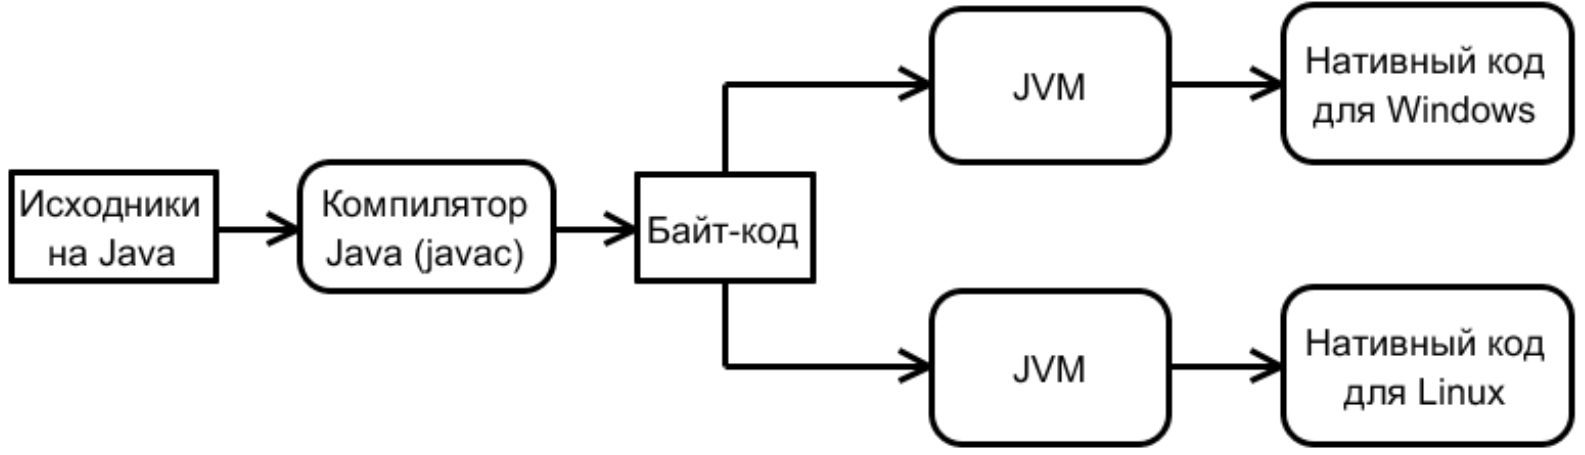
\includegraphics[width=0.9\textwidth]{javaCompiling.png}
		\end{center}
	\end{frame}

	\begin{frame}
		\frametitle{Особенности}
		\begin{itemize}
			\item Сборка мусора
			\begin{itemize}
				\item Это не значит, что за памятью можно не следить!
			\end{itemize}
			\item Практически всё --- объект
			\item Стандартизация элементарных типов (в отличие от С++)
			\item Пакеты и библиотеки (имена пакетов стандартизованы, например, com.example.myclasses)
			\item Рефлексия
			\item Некоторая поддержка функционального стиля
			\item Несколько странная реализация шаблонов (генерики)
		\end{itemize}
	\end{frame}

	\section{Типы}

	\begin{frame}
		\frametitle{Mandatory slide про стандартные числовые типы}
		\begin{tabu} {| X[0.3 l p] | X[1 l p] | X[0.2 l p] |}
			\tabucline-
			Тип       & Значения                                                                              & Размер  \\
			\tabucline-
			\everyrow{\tabucline-}
			$byte$    & $-2^7..2^7-1 (-128..127)$                                                             & 8 бит   \\
			$short$   & $-2^15..2^15-1 (-32768..32767)$                                                       & 16 бит  \\
			$int$     & $-2^31..2^31-1$                                                                       & 32 бит  \\
			$long$    & $-2^63 .. 2^63-1$                                                                     & 64 бит  \\
			$float$   & $-3.4028235E+38..-1.4E-45$ \newline и $1.4E-45..3.4028235E+38$                        & 32 бит  \\
			$double$  & $-1.7976931348623157E+308..-4.9E-324$ \newline и $4.9E-324..1.7976931348623157E+308$  & 64 бит  \\
		\end{tabu}
	\end{frame}

	\begin{frame}
		\frametitle{Ссылочные типы и типы-значения}
		\begin{itemize}
			\item Примитивные типы: \mintinline{java}|byte, short, int, long, float, double, boolean, char|
			\item Ссылочные типы: массивы, классы (в том числе строки и типы-обёртки), интерфейсы, перечисления, аннотации
			\item Ссылочные типы всегда хранятся на куче и передаются по ссылке, примитивные типы всегда хранятся и передаются по значению
			\item У каждого типа есть значение по умолчанию --- \mintinline{java}|null| для ссылочных типов (в том числе массивов и строк), нули для всех остальных
			\item Оператор == для ссылочных типов всегда сравнивает их место в памяти
			\begin{itemize}
				\item Строки нельзя сравнивать ==, используйте equals
			\end{itemize}
		\end{itemize}
	\end{frame}

	\begin{frame}
		\frametitle{Типы-обёртки, что?}
		\begin{itemize}
			\item Классы, соответствующие примитивным типам и поддержанные компилятором
			\item Boxing/Unboxing
			\item \mintinline{java}|byte| --- \mintinline{java}|Byte|, \mintinline{java}|short| --- \mintinline{java}|Short|, ну вы поняли
			\item Не всё так просто: \mintinline{java}|char| --- \mintinline{java}|Character|, \mintinline{java}|int| --- \mintinline{java}|Integer|
			\item Методы: \mintinline{java}|int ololo = Integer.parseInt("239");|
			\item Известная ``особенность'':
			\begin{itemize}
				\item \mintinline{java}|Integer.valueOf(127) == Integer.valueOf(127)|
				\item но \mintinline{java}|Integer.valueOf(128) != Integer.valueOf(128)|
			\end{itemize}
		\end{itemize}
	\end{frame}

	\section{Инструменты}

	\begin{frame}
		\frametitle{IntelliJ IDEA, демонстрация}
		\begin{center}
			\huge{Демонстрация}
		\end{center}
	\end{frame}

	\begin{frame}
		\frametitle{Что скачать и поставить}
		\begin{itemize}
			\item JDK 11 (\url{https://www.oracle.com/technetwork/java/javase/downloads/jdk11-downloads-5066655.html})
			\begin{itemize}
				\item Обратите внимание, JRE --- среда времени выполнения, JDK --- среда времени выполнения + инструменты разработки (включая компилятор)
				\item Очень желательно добавить javac в PATH и прописать переменную окружения JAVA\_HOME
			\end{itemize}
			\item IntelliJ IDEA (\url{https://www.jetbrains.com/student/})
		\end{itemize}
	\end{frame}

	\begin{frame}
		\frametitle{Что сдавать}
		\begin{itemize}
			\item Файлы .java
			\item Папку .idea
			\begin{itemize}
				\item Кроме workspace.xml, usage.statistics.xml, tasks.xml
			\end{itemize}
			\item Файлы .iml (если есть)
			\item Ничего больше
		\end{itemize}
		Решения надо выкладывать на GitHub, ссылку в HwProj
	\end{frame}

	\begin{frame}
		\frametitle{Как собирать из консоли}
		\begin{itemize}
			\item javac
			\begin{itemize}
				\item javac MyClass.java YetAnotherClass.java
				\item javac -d classes MyClass.java
				\item javac -classpath classes;library.jar -d classes MyClass.java
			\end{itemize}
			\item CLASSPATH
			\begin{itemize}
				\item Набор путей, по которым компилятор и Java-машина ищут классы
				\item Всегда содержит классы из стандартной библиотеки
				\item По умолчанию --- текущая директория (``.'')
				\item Задаётся как список директорий или JAR-файлов, через ``;'' в Windows и через ``:'' во всём остальном
				\begin{itemize}
					\item JAR-файл --- просто заархивированная папка с классами, по сути --- библиотека
				\end{itemize}
			\end{itemize}
			\item Системы сборки --- Gradle, Maven, ...
		\end{itemize}
	\end{frame}

	\begin{frame}
		\frametitle{Как запускать из консоли}
		\begin{itemize}
			\item Нет никакого .exe-шника, виртуальной машине передаётся на исполнение файл с байт-кодом класса
			\item Оный класс должен иметь метод \mintinline{java}|public static void main(String[] args)|
			\item java (javaw)
			\begin{itemize}
				\item java MyClass
				\item java -classpath classes\_dir;library.jar MyClass
				\item java -jar library\_with\_main\_class.jar
				\begin{itemize}
					\item не всё так просто, jar-нику нужен манифест
				\end{itemize}
				\item Имя запускаемого класса должно быть \textbf{полностью квалифицированным}
				\begin{itemize}
					\item например, \textit{java com.example.MyClass}
				\end{itemize}
				\item Нелишне посмотреть документацию, есть много полезных ключей командной строки
			\end{itemize}
			\item Системы сборки несколько облегчают эту боль
		\end{itemize}
	\end{frame}

	\begin{frame}
		\frametitle{Некоторые тонкости IDEA}
		\begin{itemize}
			\item Есть отдельно меню File -> Settings и отдельно File -> Project Structure
			\begin{itemize}
				\item Settings --- это в основном настройки самой среды
				\item Project Structure --- это настройки проекта
				\begin{itemize}
					\item Версия языка (есть отдельно версия языка и отдельно версия SDK)
					\item Модули --- в какой папке код, в какой тесты, в какой ресурсы; IDEA компилит только папки, отмеченные как Sources или Tests
				\end{itemize}
			\end{itemize}
			\item Справа вверху --- конфигурации запуска. Там можно настроить, например, параметры командной строки
			\item Знание основных хоткеев может спасти жизнь на контрольной
		\end{itemize}
	\end{frame}

	\section{Стайлгайд}

	\begin{frame}
		\frametitle{Стайлгайд}
		\begin{itemize}
			\item \url{https://google.github.io/styleguide/javaguide.html} (только для отступа используйте 4 пробела, а не 2)
			\item На что обратить внимание:
			\begin{itemize}
				\item camelCase для методов и ``переменных'', CamelCase для типов, КАПС\_ДЛЯ\_КОНСТАНТ
				\item Правильные имена пакетов (DNS-имя наоборот + собственно имя пакета)
				\item ``Египетские'' фигурные скобки (так же известны, как K \& R)
				\item Минимально возможная видимость полей, методов и всего-всего
				\begin{itemize}
					\item Всегда указывайте модификатор видимости
				\end{itemize}
				\item Комментарии к каждому классу и каждому public-методу
				\begin{itemize}
					\item JavaDoc
				\end{itemize}
			\end{itemize}
		\end{itemize}
	\end{frame}

	\begin{frame}
		\frametitle{JavaDoc}
		\begin{itemize}
			\item Стандартная система генерации документации
			\item В IDEA это Tools -> Generate JavaDoc
			\item \mintinline{java}|/**  */| --- JavaDoc-комментарий
			\item Сначала общее описание, затем, опционально, уточняющие тэги
			\item Тэги:
			\begin{itemize}
				\item \mintinline{java}|@param имя описание параметра|
				\item \mintinline{java}|@return описание возвращаемого значения|
				\item \mintinline{java}|@exception ИмяКлассаИсключения описание, когда бросается|
				\item \mintinline{java}|{@inheritDoc}|
				\item \mintinline{java}|@see|
			\end{itemize}
			\item Пустые тэги не очень полезны
		\end{itemize}
	\end{frame}

\end{document}
